%generare il pdf con il comando: pdflatex main.tex
\documentclass[a4paper, oneside, openany, dvipsnames, table]{article}
\usepackage{./template/SWEightStyle}
\usepackage{tabularx}
\newcommand{\mc}{\multicolumn} % handy shortcut macro
\newcolumntype{Z}{>{\centering\arraybackslash}X}
\newcommand{\Titolo}{Manuale Utente}

\newcommand{\Gruppo}{SWEight}

\newcommand{\Approvatore}{Damien Ciagola}
\newcommand{\Redattori}{Alberto Bacco \newline Sebastiano Caccaro \newline Gheorghe Isachi \newline Gionata Legrottaglie}
\newcommand{\Verificatori}{Francesco Corti \newline Francesco Magarotto}

\newcommand{\pathimg}{../template/img/logoSWEight.png}

\newcommand{\Versionedoc}{1.0.0}

\newcommand{\Distribuzione}{\proponente \newline Prof. Vardanega Tullio \newline Prof. Cardin Riccardo \newline Gruppo SWEight}

\newcommand{\Uso}{Esterno}

\newcommand{\NomeProgetto}{Colletta}

\newcommand{\Mail}{SWEightGroup@gmail.com}

\newcommand{\DescrizioneDoc}{Questo documento si occupa di fornire le modalità di utilizzo del software Colletta commissionato}

\usepackage{xcolor}
\usepackage{hyperref}
\usepackage{listings}
\usepackage{forest}
\usepackage{textcomp}

\definecolor{folderbg}{RGB}{124,166,198}
\definecolor{folderborder}{RGB}{110,144,169}

\def\Size{4pt}
\tikzset{
  folder/.pic={
    \filldraw[draw=folderborder,top color=folderbg!50,bottom color=folderbg]
      (-1.05*\Size,0.2\Size+5pt) rectangle ++(.75*\Size,-0.2\Size-5pt);  
    \filldraw[draw=folderborder,top color=folderbg!50,bottom color=folderbg]
      (-1.15*\Size,-\Size) rectangle (1.15*\Size,\Size);
  }
}

\begin{document}
\copertina{}
\newpage
\rowcolors{2}{greyROwSWEight}{white}
\section*{Change log}
{
	\renewcommand{\arraystretch}{1.5}
	\centering
	\begin{longtable}{ c c C{6cm} c c }
		\rowcolor{greySWEight}
		\textcolor{white}{\textbf{Version}} & \textcolor{white}{\textbf{Date}} & \textcolor{white}{\textbf{Description}} & \textcolor{white}{\textbf{Author}} & \textcolor{white}{\textbf{Role}}\\
		1.1.1 & 2019-05-08 & Refactor §\ref{sec:BackArchi}  & Francesco Corti & \reda{}\\
		1.1.0 & 2019-05-06 & Refactor §\ref{sec:FrontArchi} & Sebastiano Caccaro & \reda{}\\
		1.0.1 & 2019-05-06 & Fixed §\ref{fig:UMLFront} & Sebastiano Caccaro & \reda{}\\
		1.0.0 & 2019-04-10 & Document approval and release & Damien Ciagola & \RdP{}\\
		0.4.0 & 2019-04-04 & Checking & Gheorghe Isachi & \ver{}\\
		0.4.0 & 2019-04-02 & §1 completed  & Francesco Corti & \reda{}\\		
		0.3.0 & 2019-04-02 & §2 and §3 completed  & Francesco Magarotto & \reda{}\\				
		0.2.0 & 2019-04-01 & §4 completed  & Sebastiano Caccaro & \reda{}\\
		0.1.1 & 2019-04-01 & Written §4 to §4.2.1  & Sebastiano Caccaro & \reda{}\\
		0.1.0 & 2019-04-01 & Backbone translated in English & Sebastiano Caccaro & \reda{}\\
		0.0.1 & 2019-03-18 & Document backbone & Enrico Muraro & \reda{}\\
		
	\end{longtable}

}


\newpage
\tableofcontents
\newpage
\listoffigures
\newpage

\newpage
\newpage
\section{Introduction}
\subsection{Document goal}
The purpose of this document is to provide all the necessary information to extend, correct and improve Colletta.
There will be additional information regarding setting up the development environment to work in an environment that is as consistent as possible with that used
by the other members of group SWEight, but can be ignored if you only want to use part of the product.
This guide was written taking into account the Microsoft Windows and Linux operating systems. If other systems are used, compatibility issues may arise, even if it's unlikely. In this case refer to the git page. This document will grow as the product will be fully
developed.

\subsection{Product goal}
The purpose of the product is the creation of a collaborative data collection platform where users can prepare and/or perform small grammar exercises. 
The front-end of the system consists of a web application developed with React and Redux, while the back-end is a Spring Boot application written in Java, which will handle HTTP Requests sent from the front-end. 

\subsection{References}


\subsubsection{Installation references}

\begin{itemize}
\item \textbf{Git}: \url{https://git-scm.com/}
\item \textbf{Node.js}: \url{https://nodejs.org/en/}
\item \textbf{NPM}: \url{https://www.npmjs.com/}
\item \textbf{Oracle JDK}: \url{https://www.oracle.com/technetwork/java/javase/downloads/index.html}
\item \textbf{OpenJDK}: \url{https://openjdk.java.net/}
\item \textbf{Maven}: \url{https://maven.apache.org/}
\item \textbf{Lombok}: \url{https://projectlombok.org/}
\item \textbf{VSCode}: \url{https://code.visualstudio.com/} 

\end{itemize}

\subsubsection{Legal references}
\begin{itemize}
\item \textbf{MIT License}: \url{https://opensource.org/licenses/MIT}
\end{itemize}

%\subsubsection{Informative references}
	

\newpage
\section{Development Requirements}
\subsection{System requirements}
\subsubsection{Windows}
\begin{itemize}
\item [•]\textbf{CPU}: Intel X86 family;
\item [•]\textbf{RAM}: at least 2GB of RAM;
\item [•]\textbf{Disk's space}: at least 1GB;
\item [•]\textbf{Operating system}: Windows 7 or superior, 32-bit or 64-bit versions;
\item [•]\textbf{Java}: Java SE Development Kit 8;
\item [•]\textbf{Node.Js}: Node.js 10.15.1;


\end{itemize}

\subsubsection{Ubuntu}
\begin{itemize}
\item [•]\textbf{CPU}: Intel X86 family;
\item [•]\textbf{RAM}: at least 2GB of RAM;
\item [•]\textbf{Disk's space}: at least 1GB;
\item [•]\textbf{Java}: Openjdk 8;
\item [•]\textbf{Node.Js}: Node.js 10.15.1;

\end{itemize}

\subsubsection{MacOS}
\begin{itemize}
\item [•]\textbf{Mac Model}: all the models sold from 2011 onwards;
\item [•]\textbf{RAM}: at least 2GB of RAM;
\item [•]\textbf{Disk’s space}: at least 1GB;
\item [•]\textbf{Operating system}: OS X 10.10 Yosemite.
\item [•]\textbf{Java}: Openjdk 8;
\item [•]\textbf{Node.Js}: Node.js 10.15.1;


\end{itemize}

\subsection{Configuration}
%TODO

\subsection{Execution}
%TODO

\newpage
\section{Workspace Configuration}
The purpose of this chapter is to describe the tools used by \gruppo{} to develop the application.
Obviously, if you are not interested in contributing to this project but you just want to run it, you can use any editor.
\subsection{IntelliJ IDEA}
The default IDE for development is IntelliJ IDEA Community created by Jet Brains, you can use it for Java and JSX development. The commmunity edition used is free and multi-platform, it runs on Windows, MacOs and Linux.

\subsection{Visual Studio Code}
An alternative IDE is Visual Studio Code developed by Microsoft, it's free and open-source and you can use it to write Java and JSX code. There are some plugins created from Pivotal and RedHat which allow you to have an environment similar to IntelliJ IDEA.

\subsection{Maven}
To manage the project you need Maven. It downloads all the dependencies including Spring Boot, compiles the source code and finally runs the application. Maven is written in Java, so you just need the Oracle JDK or the OpenJDK at least version 8.

\subsection{React}
To better debug React components it is recommended to use the following plugins:
\begin{itemize}
\item \textbf{Mozilla Firefox}(current version 66): \\
\url{https://addons.mozilla.org/it/firefox/addon/react-devtools/};
\item \textbf{Google Chrome}(current version 73): \\
\href{https://chrome.google.com/webstore/detail/react-developer-tools/fmkadmapgofadopljbjfkapdkoienihi}{https://chrome.google.com/webstore/detail/react-developer-tools/}
\end{itemize}
Remember to disable cache in the browser during the development.

\subsection{Redux}
To better debug in Redux it is recommended to use the plugin available at \url{https://extension.remotedev.io/} which can be used as extension in Google Chrome 73 and Mozilla Firefox 66.

 



\section{General structure}
\begin{figure}[H]
\centering
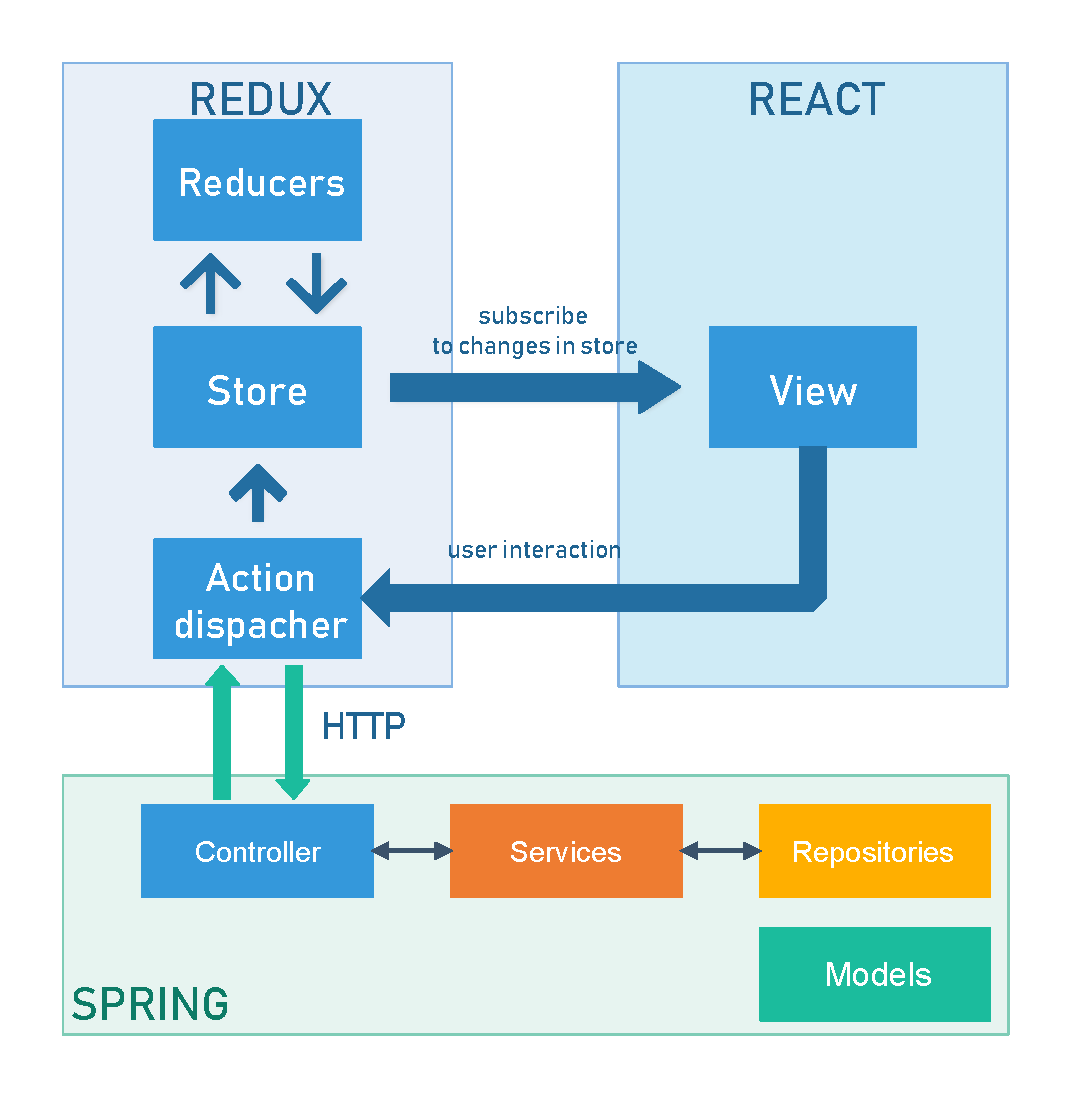
\includegraphics[]{uml/general.pdf} 
\caption{General schema of the application}
\label{fig:Archi}
\end{figure}

\autoref{fig:Archi} contains the overview of the application architecture. The software package uses React-Redux for the Frontend which communicates with a Springboot based Backend via REST calls.\\
A more detailed view at the architecture can be found in \autoref{sec:FrontArchi} and @@@@@@@@@@@@Riferimento architettura backend@@@@@@@@@@@@.

\newpage
\section{Frontend} %Non sono parole staccate, o scrivete Frontend o Front-End ma non mi pare il caso
\label{sec:Frontend}
This section is intended to make the developer understand the inner workings of the Colletta frontend, and to allow him or her to add more functionality to the software package.
In order fully understand the contents below, the developer must have a certain degree of familiarity with React and Redux. If that's not the case, we strongly recommend the reader to at least acquire some basic knowledge on the topics.
\subsection{Architecture}
\label{sec:FrontArchi}
In \autoref{fig:UMLFront}, one can have a glimpse into the general architecture of the Frontend of the software package.
Although it may seem quite complex at first, the architecture is actually just a more expanded version of the basic Redux patter in \autoref{fig:Redux}:
\begin{itemize}
	\item Reducers, Actions and Views are grouped by logical function to increase code readability and reduce pairing;
	\item Helpers and Constants are declared to deal with minor logic which cannot be dealt with in the Backend.
\end{itemize}

\begin{figure}
\centering 
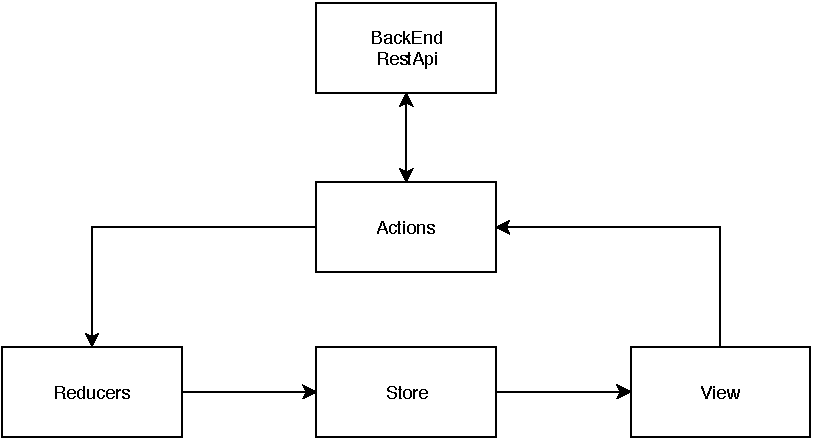
\includegraphics[width=12cm]{uml/Flux.pdf} 
\caption{Basic Redux architecture}
\label{fig:Redux}
\end{figure}

\begin{figure}
\centering 
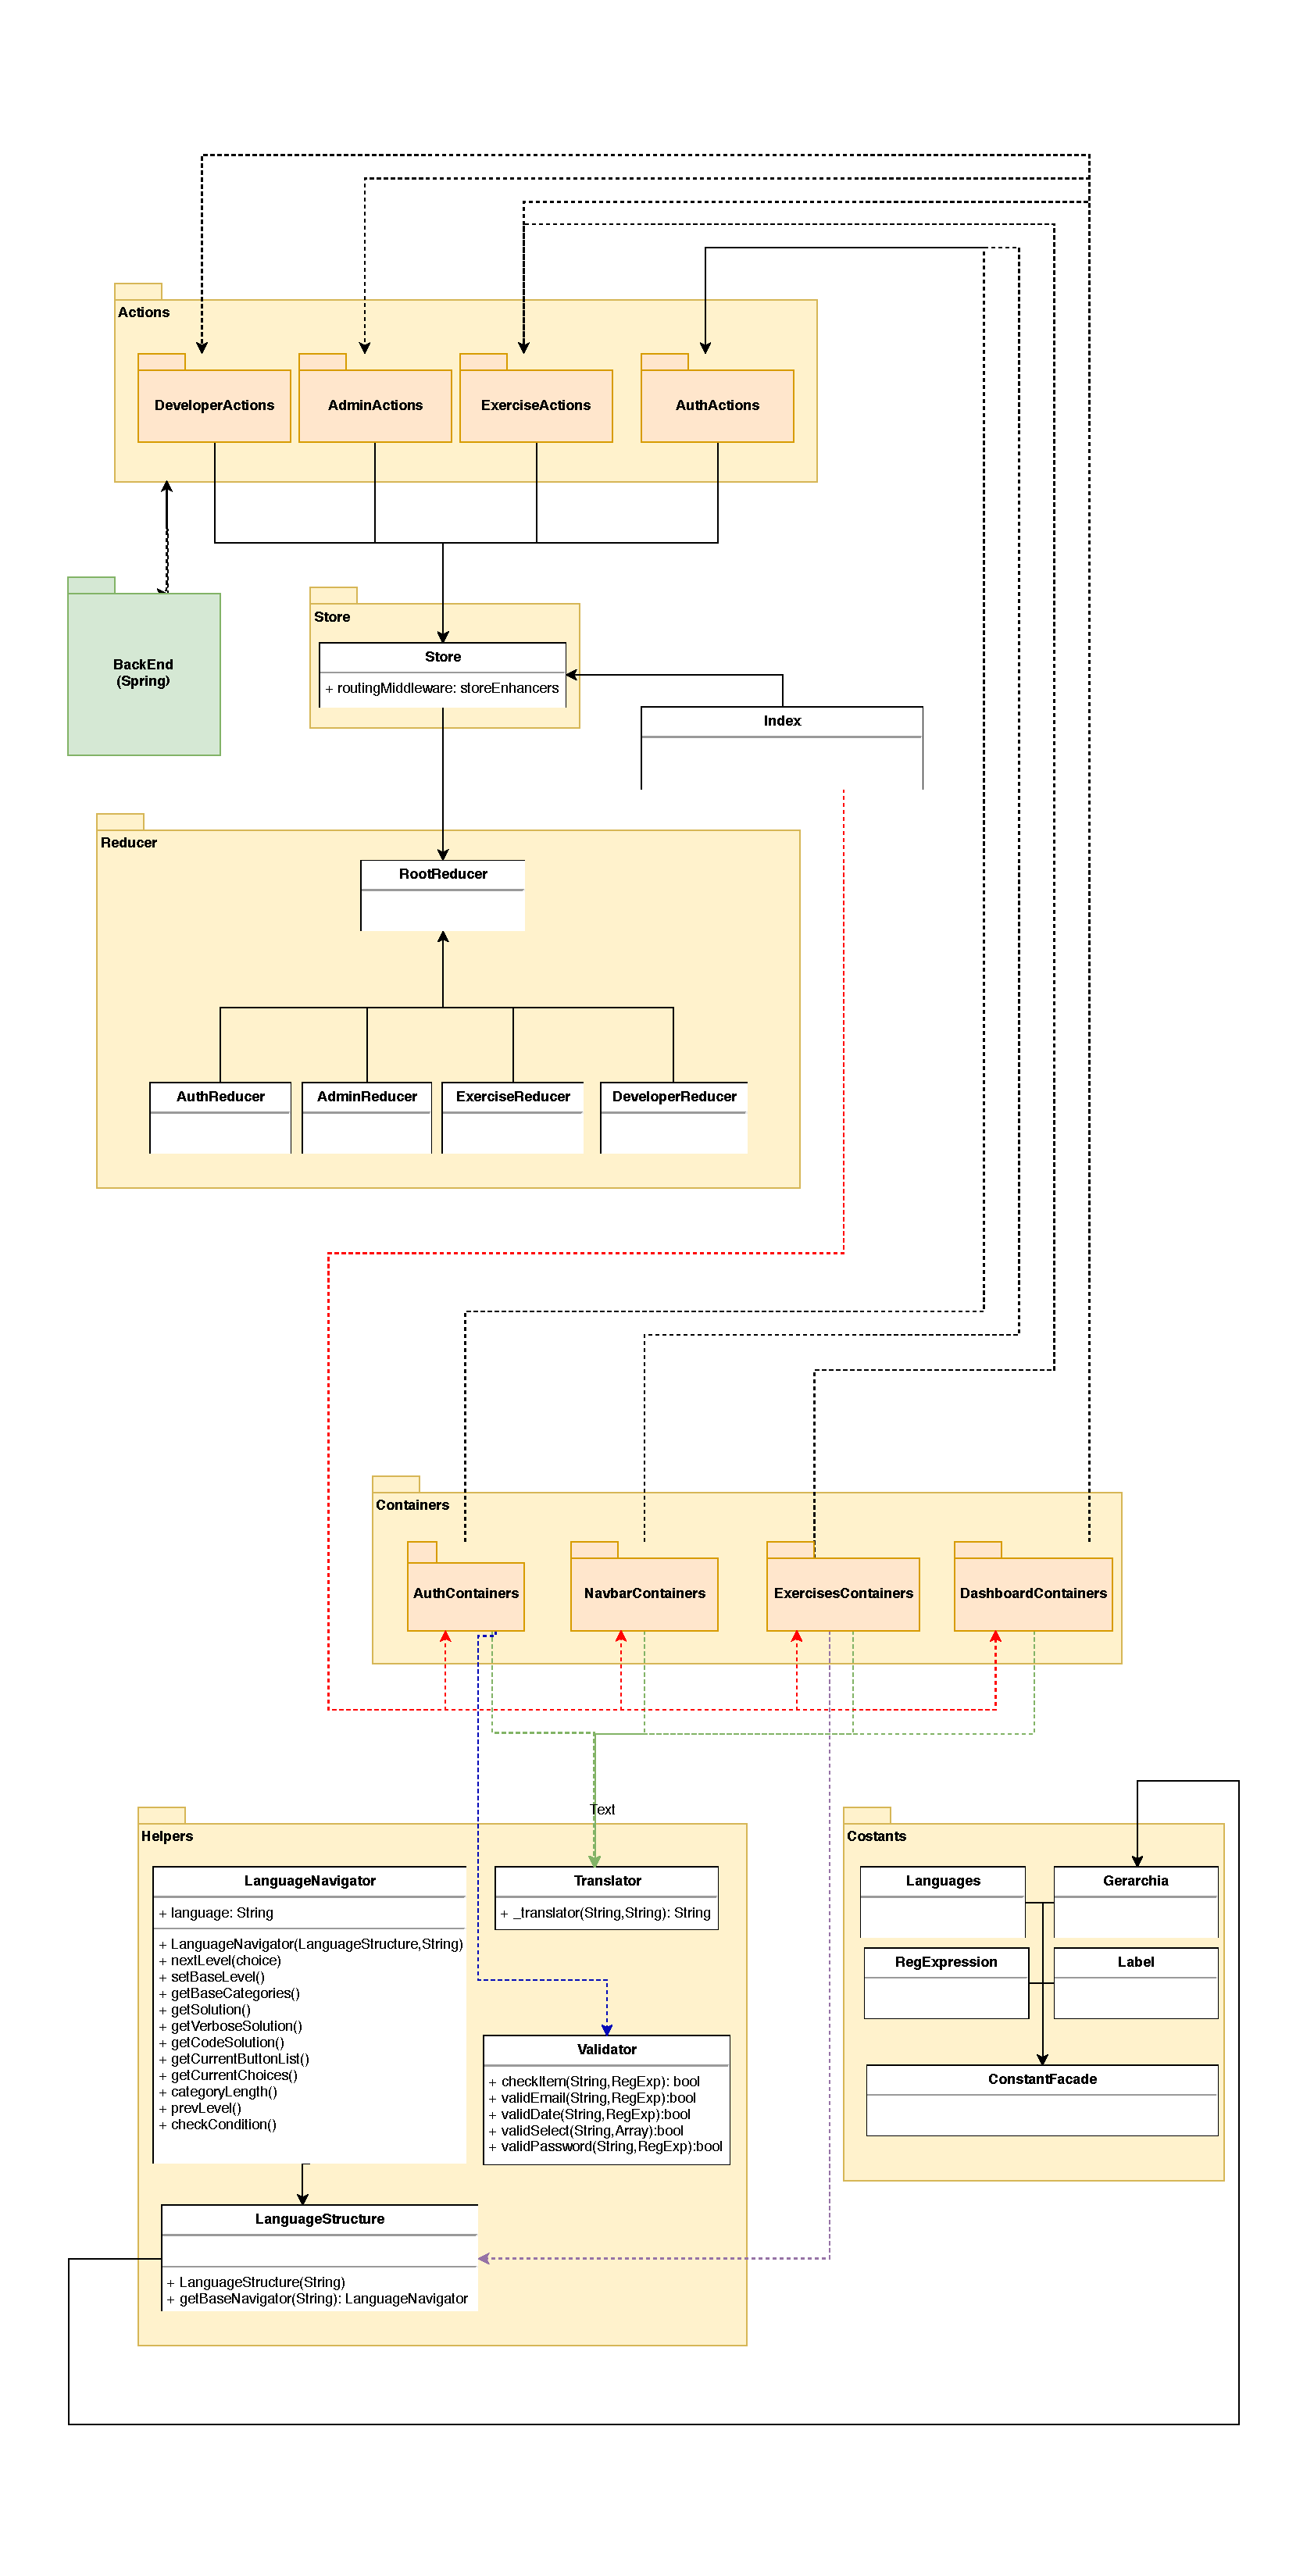
\includegraphics[width=15cm, height=18cm]{uml/reactredux.pdf} 
\caption{React and Redux architecture}
\label{fig:UMLFront}
\end{figure}
\subsection{Directory tree}
\begin{figure}[H]
\centering
\begin{forest}
  for tree={
    font=\ttfamily,
    grow'=0,
    child anchor=west,
    parent anchor=south,
    anchor=west,
    calign=first,
    inner xsep=7pt,
    edge path={
      \noexpand\path [draw, \forestoption{edge}]
      (!u.south west) +(7.5pt,0) |- (.child anchor) pic {folder} \forestoption{edge label};
    },
    before typesetting nodes={
      if n=1
        {insert before={[,phantom]}}
        {}
    },
    fit=band,
    before computing xy={l=15pt},
  }  
[Frontend
	[src
		[actions
		]
		[assets
		]
		[constants
		]
		[helpers
		]
		[reducer
		]
		[store
		]
		[view
			[containers]
			[components]
		]
	]
]
\end{forest}
\caption{Frontend directory tree}
\label{fig:BackDir}
\end{figure}

Each folder contains a specific set of files:
\begin{itemize}
	\item \textbf{actions:} the modules in this folder are responsible for creating and dispatching the actions to the reducers;
	\item \textbf{assets:} static files like font and images;
	\item \textbf{constants:} data collections and constants used in various parts of the code, i.e. the label used for the translation;
	\item \textbf{helpers:} standard js functions or classes which have some use in the code, i.e. the label translator;
	\item \textbf{reducers:} all the reducers responsible for the creation of a new state;
	\item \textbf{store:} a single file creating and giving access to the centralized state;
	\item \textbf{view:} classes rendering the information in the store. They are divided in \textit{components} and \textit{containers}.	 The key point to bear in mind when talking about components and containers is the following: containers are "smart", they observe the store and can call actions; components, on the other hand, are basically just static functions.
\end{itemize}

\subsection{Modify or add features}
\subsubsection{Components}
Components extend the React \texttt{component} abstract class and implement the \texttt{render()} method. They can be viewed as a pure functions of the props passed by their father component or container. They do not have access to the store. When adding or modifying a component the following rules should be followed:
\begin{itemize}
	\item Since the global state of the application is managed by Redux, do not use or create the local state of the component. Instead, rely solely on the props;
	\item Helper functions may be defined in the component class, but none of them should call action creators or external resources such as API calls;
	\item All components must be placed in the \texttt{src/component} folder;
	\item Every component which needs to render some text must have a language prop to call to the translator module;
\end{itemize}
When adding a new component, one can start from the following snippet:
\begin{lstlisting}[language=JavaScript, frame=single]
import React, { Component } from 'react';
import _translator from '../../helpers/Translator';
class SampleComponent extends Component {

  render() {
    const { prop1,prop2,prop3 } = this.props;
    //Do stuff here
    return (
      <React.Fragment>
        {/* Stuff to render */}
      </React.Fragment>
    );
  }
}
export default SampleComponent;
\end{lstlisting}


\subsubsection{Containers}
Containers extend the React \texttt{component} abstract class and implement the \texttt{render()} method. They can read the store and alter its state via actions. Containers can also have props passed to them, just like a container. When adding or modifying a component the following rules should be followed:
\begin{itemize}
	\item Since the global state of the application is managed by Redux, do not use or create the local state of the container. Instead, rely solely on the props and on the store;
	\item The store and the actions should not be accessed directly for performance and readability reasons. Instead, they should be mapped to the props;
	\item All containers must be placed in the most appropriate \texttt{src/view/containers} sub-directory. Creation of new sub-directories is allowed if necessary.
\end{itemize}

When adding a new container, one can start from the following snippet:
\begin{lstlisting}[language=JavaScript, frame=single]
import React, { Component } from 'react';
import { connect } from 'react-redux';
import _translator from '../../../helpers/Translator';

class SampleContainer extends Component {

  render() {
    const { prop1, prop2, prop3, action1Prop, action2Prop } = this.props;
    // Do stuff
    return (
      // Stuff to render
    );
  }
}
const mapStateToProps = store => {
  return {
    prop1: store.object1,
    prop2: store.object2,
    prop3: store.object3
  };
};

const mapDispatchToProps = dispatch => {
  return {
    action1Prop: () => dispatch(action1()),
    action2Prop: () => dispatch(action2())
  };
};
//both action1 and action2 must be imported

export default connect(
  mapStateToProps,
  mapDispatchToProps
)(SampleContainer);
\end{lstlisting}


\subsubsection{Rest API calls}
When implementing a new Rest API call (RAP from now on), the developer must stick to the following guidelines:
\begin{itemize}
	\item RAPs must be implemented inside an action creator and should not be put inside components or containers;
	\item RAPs must use the Axios module;
	\item RAPs must pass an authorization token (exception made for Log-in and Sign-up) which is kept in the store. The snippet below will show clarify how;
	\item If a RAP does not need additional data, the data field should be replaced by \texttt{\{\}}, otherwise the response will display a 403 error.
\end{itemize}
When adding a new RAP, one can start from the following snippet:
\begin{lstlisting}[language=JavaScript, frame=single]
export const sampleActionCreator = objectToSend => {
  return dispatch => {
    axios
      .post(
        'http://localhost:8081/sample-call',
        {
          ...objectToSend
        },
        {
          headers: {
            'content-type': 'application/json',
            Authorization: store.getState().auth.token
          }
        }
      )
      .then(response => {
        // Maybe do something
        dispatch({ type: 'SAMPLE-ACTION', dataToDispatch });
      })
      .catch(() => {/* Handle Error Here*/});
  };
};
\end{lstlisting}


\subsubsection{Interface Language}
The multiple languages of the application are implemented via the Translator module in the \texttt{src/helpers} folder. Every single piece of text shown to the user is stored in \texttt{src/constants/Label.js} in all the languages supported by Colletta. Each language is identified by its ISO 639-1 code.\\
Each string variable is composed as follow:
\begin{center}
context\_identifier
\end{center}
where:
\begin{itemize}
\item \textbf{Context} is the component or container in which the string is used. If it is used in more than one component or container, context should be \texttt{gen}. Context must start with a lowercase letter;
\item \textbf{Identifier} should sum up the function of the string. It must start with a lowercase letter.
\end{itemize}
The translated string can than be displayed with the following function:
\begin{center}
\texttt{\_translator('string\_variable', language)}
\end{center}
where:
\begin{itemize}
\item \textbf{String\_variable} is the name of the string you want to render. It must be surrounded by single quotes;
\item \textbf{Language} is a string containing the ISO 639-1 code of the language you want to render the string in.
\end{itemize}
Therefore, whenever one wants to add some new text to some component or container, he or she must add the string in all of the supported languages and render it with the translator module.\\
If instead one wants to implement a new language, the following steps need to be followed:
\begin{enumerate}
\item Every single string in \texttt{Label.js} must be translated and inserted with the ISO 639-1 code of the language;
\item The variable \texttt{UiLang} in \texttt{src/constants/Label.js} must be updated with the ISO 639-1 code of the language;
\item For every language in \texttt{Label.js}, a string in the format \texttt{gen\_xx} must be added, with xx being the ISO 639-1 code of the language. The string must contain the language name. For instance, in English \texttt{gen\_it} is Italian and \texttt{gen\_en} is English.
\end{enumerate}
The following snippet represents a slim-down example of \texttt{Label.js}:
\begin{lstlisting}[language=JavaScript, frame=single]
export const _label = {
  it: {
    account_yourData: 'I tuoi dati',
    dashboard_hiUser: 'Ciao, ',
    executionExercise_complete: 'Completa',
    gen_it: 'Italiano',
    gen_en: 'Inglese'
  },
  en: {
    account_yourData: 'Your data',
    dashboard_hiUser: 'Hello, ',
    executionExercise_complete: 'Submit solution',
    gen_it: 'Italian',
    gen_en: 'English',
  }
};
\end{lstlisting}


\subsubsection{Analysis Languages}
The process for enabling other analysis languages is a little bit more tedious, as it means having to work with the Freeling tagset.
Let's have a brief overview at what needs to be done:
\begin{enumerate}
\item A custom {JSON}\textsubscript{G} tagset must be created starting from the Freeling tagset;
\item The tagset created must be modified to accommodate some conditions;
\item The tagset must be placed in the correct folder.
\end{enumerate}
One can find the {Freeling}\textsubscript{G} tagsets and their description at: \href{https://talp-upc.gitbook.io/freeling-4-1-user-manual/tagsets}{freeling-4-1-user-manual}. Starting from the tables in the Freeling doc, the end result should look like this:
\begin{lstlisting}[language=JavaScript, frame=single]
const italian = {
  adjective: {
    text: { full: 'adjective', short: 'A' },
    attributes: [
      {
        attrName: 'type',
        choices: [
          { short: 'O', full: 'Ordinal' },
          { short: 'Q', full: 'Qualifying ' },
          { short: 'P', full: 'Possessive' }
        ],
        condition: null
      },
      {
        attrName: 'degree',
        choices: [
          { short: 'S', full: 'superlative' },
          { short: '0', full: 'none' }
        ],
        condition: { index: 1, short: 'Q' }
      },
      //...........
\end{lstlisting}
Let's break in down:
\begin{itemize}
\item The outermost level contains the categories of word in the language (i.e. adjective, noun, etc...);
\item Each category has a text value, a name, a condition, and a list of choices. Each choice represents a possible value for the attribute.
\item Choices and text objects of attributes contain two string:
	\begin{itemize}
	\item \textbf{Full}: the name of the choice or category (i.e. Adjective, Ordinal).
	\item \textbf{Short}: the letter corresponding to the choice or the category (i.e. Adjective is A, Ordinal is O.
	\end{itemize}
\end{itemize}
The modifications which have been made from the standard tagset are the following:
\begin{itemize}
\item \textbf{Conditions}: this field is needed to avoid showing the user choices that cannot be taken. For instance, it would make no sense to show the option to select the superlative option if the adjective selected has been marked as possessive. Thus, the condition states that the attribute at \texttt{index: 1} must have \texttt{short: Q}, so it must be qualifying. If no restriction applies, the condition field must be set to null;
\item \textbf{None fields}: looking at the code example above, one may notice the following choice: \texttt{\{ short: '0', full: 'none' \}}. It has been added to let the user to mark an adjective as not superlative. This choice must be added whenever an attribute is not strictly mandatory.
\end{itemize}
Adding conditions and none fields requires a decent understanding of the grammar of a language, and it is a process that must be executed very carefully.\\
Once the file is completed, it can be placed in the \texttt{src/constants} folder, named as \texttt{ger\_xx} where \texttt{xx} is the ISO 639-1 code of the language.\\
Disclaimer: Freeling documentation is not always reliable. The tagset might be incomplete or contain some errors.








%%sia front end che backend devono avere una descrzione dell'archietettura, e poi descrivere come 
%%estendere il tutto. Vedi marvin (con correzioni)

\newpage
\section{Backend}
%Non sono parole staccate, o scrivete Backend o Back-End ma non mi pare il caso
This section is intended to make the developer understand the working of the Colletta backend, and to allow him or her to add functionalities  to the software package.
In order to fully understand the contents below, the developer must have a certain degree of familiarity with Java, the framework Spring Boot with his subframework Spring Data MongoDB, MongoDB and Maven. If that's not the case, we strongly recommend the reader to at least acquire some basic knowledge on the topics.

\subsection{Directory tree}

\begin{figure}[H]
\centering
\begin{forest}
  for tree={
    font=\ttfamily,
    grow'=0,
    child anchor=west,
    parent anchor=south,
    anchor=west,
    calign=first,
    inner xsep=7pt,
    edge path={
      \noexpand\path [draw, \forestoption{edge}]
      (!u.south west) +(7.5pt,0) |- (.child anchor) pic {folder} \forestoption{edge label};
    },
    before typesetting nodes={
      if n=1
        {insert before={[,phantom]}}
        {}
    },
    fit=band,
    before computing xy={l=15pt},
  }  
[Backend
	[src
		[main 
			[java
				[it
					[colletta
						[controller]
						[error]
						[exceptions]
						[library]
						[model
							[helper]
						]
						[repository]
						[security]
						[service]						
					]
				]
			]
			[resources]
		]	
		[test
			%[it
			%	[colletta
			%		[repository
			%			[config]
			%			[exercise]
			%			[phrase]
			%			[user]
			%		]
			%		[service
			%			[user]
			%		]
			%	]
			%]
		]				
	]
]
\end{forest}
\caption{Backend directory tree}
\label{fig:FrontDir}
\end{figure}

Each folder contains a specific set of files:
\begin{itemize}
\item  \textbf{controller}: classes that handle HTTP Request, marked with \textit{@RestController} Spring annotation;
\item  \textbf{error}: custom class for error handling;
\item  \textbf{exceptions:} custom class for exception handling;
\item  \textbf{library}: classes that connect the application to the PoS-tagging library;
\item  \textbf{model}: has the folder \textit{helper} which contains the transfer object (DTO), the other Model files are standard POJO objects that represent JSON objects store inside the database;
\item  \textbf{repository}: classes that encapsulates the set of objects persisted in a data store, in our case MongoDB, and the operations performed over them, providing a more object-oriented view of the persistence layer;
\item  \textbf{security}: classes that manages the security of the application through encryption and token management;
\item  \textbf{service}: classes that make up the logical business part of the application;
\item  \textbf{test}: the tests that the application must pass to enter in a safe running state;
\item \textbf{resources}: contains the configuration file for connection to the database.
\end{itemize}

\subsection{Data and logic separation}
\begin{figure}[H]
\centering 
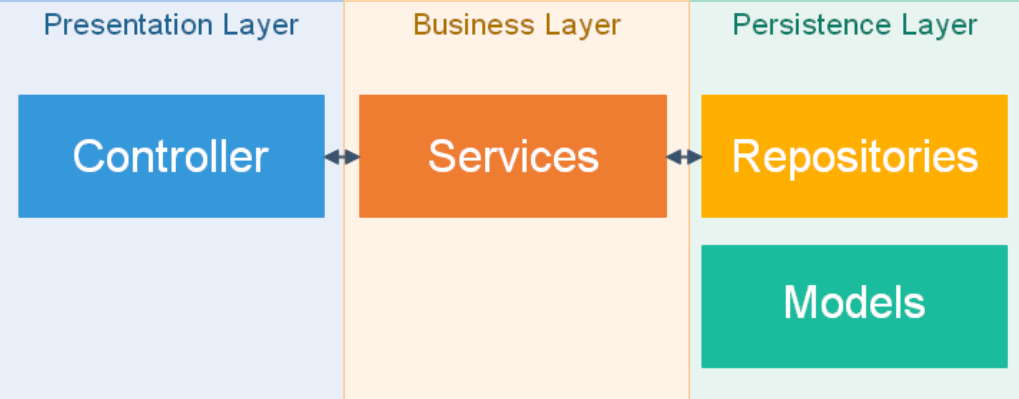
\includegraphics[scale=0.3]{uml/backendArchitecture.png} 
\caption{Data and logic separation}
\end{figure}

The design pattern used for the backend is: \textbf{Spring MVC}.
Respectively with the Controller, Service and Repository classes.
\\ 
To get more information about the architecture chosen for the backend, follow the link below: \href{https://docs.spring.io/spring/docs/current/spring-framework-reference/web.html}{Spring Web MVC}.


\subsection{Security}
The system was designed to secure client server communication so that only a user registered in the system can make calls which are then resolved by interacting with the database.\\
In authentication, when the user successfully logs in using their credentials, a JSON Web Token will be returned, instead if the user has registered the token will be generated.\\
Whenever the user wants to access a protected route or resource he/she must necessarily send his token that identifies he/she as a user correctly registered in the system. If this is not done the system will decline the request.\\
The security system has been implemented so that the only requests that are authorized without token recognition are the login (\textit{/login}) and the registration (\textit{/sign-up}).\\
The system uses \textit{JWT tokens} for token authentication, more information is available at the link: \href{https://jwt.io/introduction/}{Introduction to JSON Web Tokens}.

\subsection{Modify or add features}
\subsubsection{Controller}
Controller has the words \textit{@RestController}, a convenience annotation which contains within it \textit{@Controller} and \textit{@ResponseBody}, above the class definition and contains the methods that map the HTTP calls sent from the frontend, being handled by the \texttt{DispatcherServlet}.\\
This configuration returns to the frontend a JSON file, if this does not want to be done the @RestController word must be replaced by \textit{@Controller}.\\
When adding a controller the following rules should be followed:
\begin{enumerate}
\item New controller must have the word \textit{@RestController} above its definition;
\item Each mapping must be unique in the application. If not, Spring throws a \texttt{RuntimeException} during application initialization. You cannot even use parameters to differentiate your endpoints;
\item The name of the controller should be significant;
\item The controller \textbf{only} needs to \textbf{handle HTTP Requests}, any kind of input control must be performed in the service that will then be called;
\item The services should be instantiated with the \textit{@Autowired} keyword, see \href{https://www.baeldung.com/spring-autowire}{Guide to Spring @Autowired} for more info, over all the methods.
\item Each method must contain the signature: @RequestMapping (value = "/", method = Request.RequestType)
\end{enumerate}
When adding a new \textit{Controller}, one can start from the following structure/example:
\begin{lstlisting}[language=Java]
@RestController
public class UserController{

	@Autowired
	UserService service; 
	
	@RequestMapping(value = "/exercises/student/do", method = RequestMethod.POST, produces = MediaType.APPLICATION_JSON_VALUE)
	public ResponseEntity<Object> doExercise(){
			//call a generic service
	}
}
\end{lstlisting}
\subsubsection{Service}
Service has the words \textit{@Service} to indicate that the class holding the business logic.\\
The service takes care of \textbf{checking} and \textbf{validating} the \textbf{inputs} sent by the frontend, if incorrect data are sent the service takes care of generating an exception that will be managed by the \textit{Controller} class.\\
When adding a service the following rules should be followed: 
\begin{enumerate}
\item A service can only call its repository;
\item All database read and write operations must be performed from the
\end{enumerate}
When adding a new \textit{Service}, one can start from the following structure/example:
\begin{lstlisting}[language=Java]
@Service
public class UserService{

	@Autowired
	UserRepository userRepository; 
	
	public List<String> findAllExerciseToDo(String userId){} 
}
\end{lstlisting}

\subsubsection{Repository}
\subsubsection{Model}


\newpage

\appendix
\addcontentsline{toc}{part}{Appendices}

\newpage
\section{Glossary}

\section*{F}
\textbf{Freeling}: the library for pos-tagging developed by TALP Research Center written in C++;
\section*{P}
\textbf{Pos-tagging}: part-of-speech tagging, also called grammatical tagging or word-category disambiguation, is the process of marking up a word in a text (corpus) as corresponding to a particular part of speech; \\ 
\textbf{POJO}: Plain Old Java Object, is an ordinary Java object, not bound by any special restriction and not requiring any class path. In Spring it refers to a Java object (instance of definition) that isn't bogged down by framework extensions;
\section*{J}
\textbf{JSON}: JavaScript Object Notation, is a lightweight data-interchange format.  It is easy for humans to read and write. It is easy for machines to parse and generate.\\
\textbf{JWT}: JSON Web Token, a JSON-based open standard (RFC 7519) for creating access tokens that assert some number of claims;


\end{document}
